\chapter{Model Development}
\label{chap:model-dev}

In this chapter I describe development a ML emulator of high-resolution climate model.
I cover the choices such as data used as target and input variables, how the data is transformed before being used by the emulator's underlying ML model and in the design and training of this ML model and inputs to the model.

\section{Data}

\subsection{\acrshort{ukcp} Local and Met Office \acrshort{uk} \acrshort{cpm}}

I aim to emulate the Met Office \acrshort{uk} \acrshort{cpm}.
This dynamical model has a grid spacing of 2.2km covering the \acrshort{uk}.
To provide boundary conditions for the  \acrshort{uk} \acrshort{cpm}, Met Office \acrshort{gcm} simulations with 60km grid spacing are first dynamically downscaled using a 12km \acrshort{rcm} \parencite{kendon2021ukcpscienceupdate}. The domain for the 12km \acrshort{rcm} is the EURO-CORDEX grid \parencite{eurocordexdomain} which covers Europe and parts of the North Atlantic and North Africa (see \url{https://cordex.org/domains/cordex-region-euro-cordex/} for full definition). Data from the \acrshort{rcm} simulation is ingested to provide boundary conditions for the UK CPM.

I use data from 12 ensemble members. Each member uses a \acrshort{gcm}/\acrshort{rcm} pair with unique parameter settings, but an identical \acrshort{cpm}. The simulations follow the \acrfull{rcp85} climate forcing scenario. I use data from three time periods provided in the initial 2021 release of \acrshort{ukcp} Local, which we refer to as ``Historic'' for 1981--2000, ``Present'' for 2021--2040 and ``Future'' for 2061--2080. This gives a total of 720 years of data.

The simulations use a 360-day year, consisting of twelve 30-day months.
A year runs from 1st December to 30th November (so 1981 means 1st December 1980 to 30th November 1981). The simulations use a 360-day year, 12 months each with 30 days. Seasons are defined as Winter: \acrfull{djf}; Spring: \acrfull{mam}; Summer: \acrfull{jja}; Autumn: \acrfull{son}.
There are 12 CPM ensemble members, each with a corresponding driving GCM ensemble member.

All data is daily means.

\subsection{Target: Precipitation}

* Coarsen to 8.8km (PSD plot?)
* 64x64 patch: to fit on easily available commodity GPU; to cover a large enough area to make samples easier to interpret (and contain some of the more complex spatial structures).
* Differences between all 12 ensemble members (distribution plot)
* Reducing skew
* Lack of correlation between CPM and GCM (correlation plot)

Precipitation is a difficult variable to model due to its high variability and complex spatial structures.
It is also a useful variable to model as it is important for many applications that have a large impact on people's lives such as flooding.
The also CPM has many improvements to the precipiation modelled to that from the driving GCM \parencite{kendon2012vhrrcmprecip, kendon2014heaviersummerrain, kendon2020futureCPMwinterprecip}.
For these reasons we choose daily mean precipitation as the first target output of our emulator.

For our target high-resolution precipitation, we coarsen the CPM output to 8.8km grid spacing using conservative interpolation and extract the England and Wales domain. The scale of resolved features in dynamical climate models is generally several times the grid box spacing \parencite{klaver2020effectiveresolution}, so this coarsening captures the better resolved scales. This coarsening also allows a good trade off between resolution and domain size and compute requirements.
This resolution (both spatial and temporal) is fine enough to be useful climate impacts assessment. For example, it is finer than that used by \textcite{bates2023ukfloodingrisk} in their state-of-the-art UK flood risk modelling.
At this resolution a 64x64 grid section covers a large enough that visualisations are intelligible to experts.
The emulator can run well on commodity hardware such as a 10GB NVIDIA GeForce RTX 2080 Ti graphics processing unit with grids 64x64 in size.

\section{Methods}

\textcite{rampal2024mlclimdownscalingreview} find both nongenerative CNN approaches like U-Net \parencite{ronnenberger2015unet} and deep generative approaches to be effective in the domain on climate downscaling.
The downscaling problem is an inherintly stochastic problem as there are many possible high-resolution states that are consistent with any coarse resolution state.

\subsection{U-Net}

\textcite{Ronneberger2015unet} and other uses in ML 4 weather and climate

\subsection{Diffusion}

\textcite{song2021sbgmsde}

\begin{figure}[ht]
	\centering
	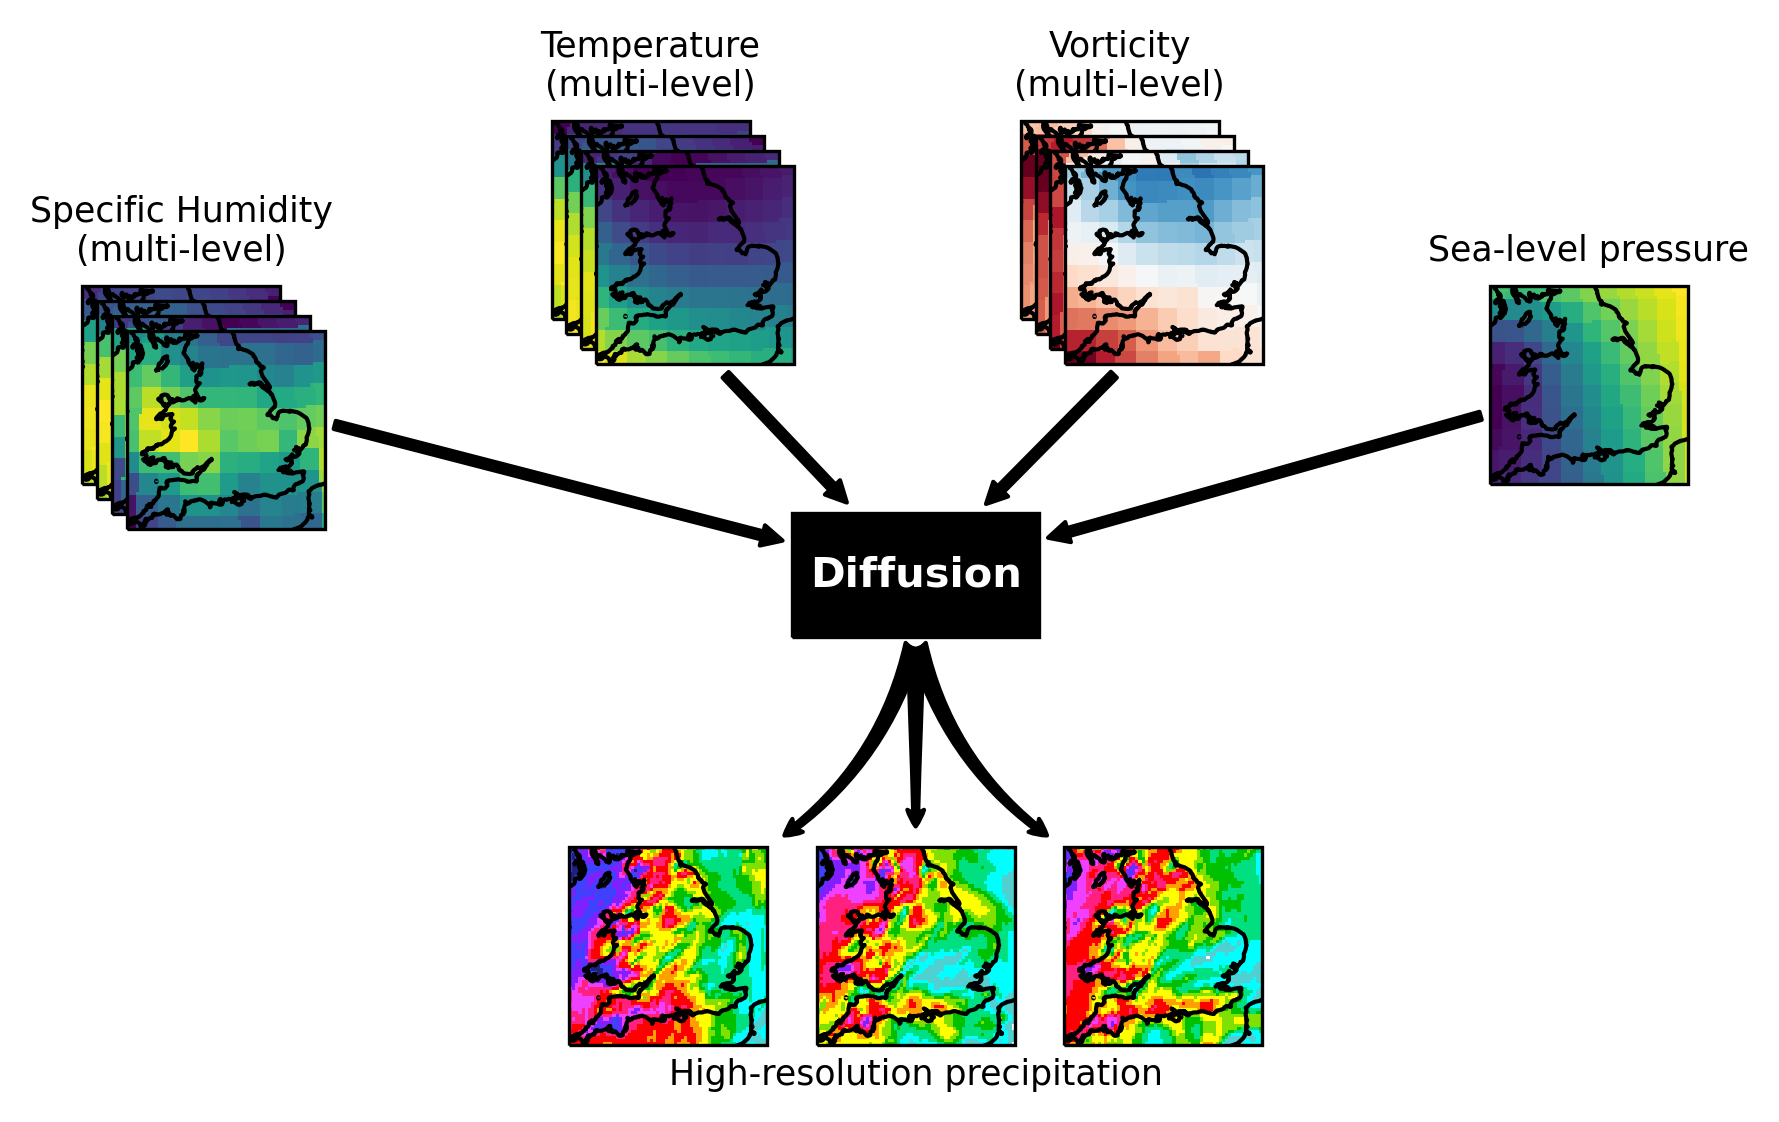
\includegraphics[height=0.35\textheight]{chapters/figures/1_intro/ai-schematic.png}
	\caption{CPM precip emulator schematic. Figure reproduced from \cite{Addison2024diffcpmprecipemul}.}
	\label{fig:diff-schematic}
\end{figure}

\section{Training}

\subsection{Dataset splits}

Variables from the same source simulation are joined on time and ensemble member. This dataset is then divided into train, validation and test splits by selecting seasons at random. This is done in a stratified way so that in a split, there are same number of each season from each of the three time periods. For example, test split is 3 randomly chosen winters from each time period and likewise for springs, summers and autumns (but not necessarily from the same years as the other seasons). This results in the following sized splits:

\begin{itemize}
    \item Train (70\%): 14 of each season from each time period (15120 days from each of the 12 ensemble members, so 181440 simulated days)
    \item Validation (15\%): 3 of each season from each time period (3240 days from each of the 12 ensemble members, 38880 simulated days)
    \item Test (15\%): 3 of each season from each time period (3240 days from each of the 12 ensemble members, 38880 simulated days)
\end{itemize}

The dataset is divided into training, validation and test subsets.
The training dataset was used to fit the model parameter values (including for transforming the variables, described below). Results for different emulator designs (e.g. choices of predictor variables and transformations) were checked on the validation dataset and used to select the final version. In this chapter, unless started otherwise, results are based on the validation dataset while I develop the emulator. I will use the test split in later chapters to give an unbiased estimate of the emulator's quality once I have settled on our final design.

For each 20 year time period, the training dataset includes 14 years in total (70\%) and the validation and test datasets include 3 years each (15\%). This is done by selecting whole seasons (Spring, Summer, Autumn and Winter) at random, with an equal number of each season in each subset. For each selected season I take data from all 12 CPM ensemble members, so that each subset has equal proportions across the ensemble members. For example, the test dataset is formed of three randomly chosen springs, summers, autumns and winters from each time period. Selecting data by season rather than day prevents data leakage between the training, validation and test datasets due to auto-correlation between days, but also means the data in each subset cover a wide range of years and sample a representative set of climatic conditions, following \textcite{schulz2021dlvsnumweather}.

\subsection{Stabilizing validation loss}

The validation loss for a diffusion model can be unstable between epochs because the loss calculation involves both sampling from the noise scales and the initial noise distribution.
Therefore from epoch-to-epoch the validation loss can vary significantly (\autoref{fig:md:unstable-val-loss}) but without indicating a significant change in the model's performance, rather than some noise scales and initial noise samples are harder to get right than others.
This is also an issue for the training loss but in practice it is less of an issue.
Perhaps, because the larger training set size means there is less dependence on the noise scales and initial noise samples each epoch.
It would also be unwise to limit the choice of noise scales and initial noise samples in the same way when training as this could lead to poor performance on certain noise scales or initial noise samples that are not so well covered during training.
To solve this for the validation loss, I used the same samples of noise scales and initial noise for each epoch in order to ``stabilize'' the calculation and get loss curves that change more smoothly from epoch to epoch.
Another alternative would be a larger validation set.

Without the stochastic component this is issue does not affect the U-Net models.

\begin{figure}
  \centering
  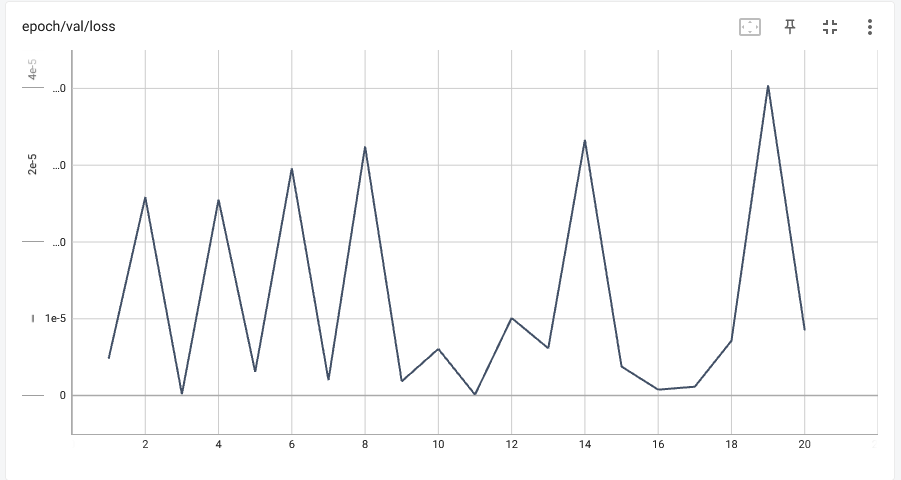
\includegraphics[width=\textwidth]{chapters/figures/3_md/loss/unstable-pr-12em-pslS4T4V4-val-loss.png}
  \caption{Unstable validation loss when different noise scales and initial noise samples are chosen at random each epoch}
  \label{fig:md:unstable-val-loss}
\end{figure}


\subsection{Stopping criteria}

With the validation loss stabilized, we can see when models start of overfit and select a checkpoint based on epochs where the validation loss is small.

With the reduced inputs and ensemble members, the 1em V850 model shows signs of overfitting once beyond the 100th-140th epoch, see \autoref{fig:md:loss}. The validation loss is unchanging between these epochs but clearly increasing again with more epochs.

\begin{figure}
  \centering
  \begin{subfigure}[b]{0.4\textwidth}
    \centering
    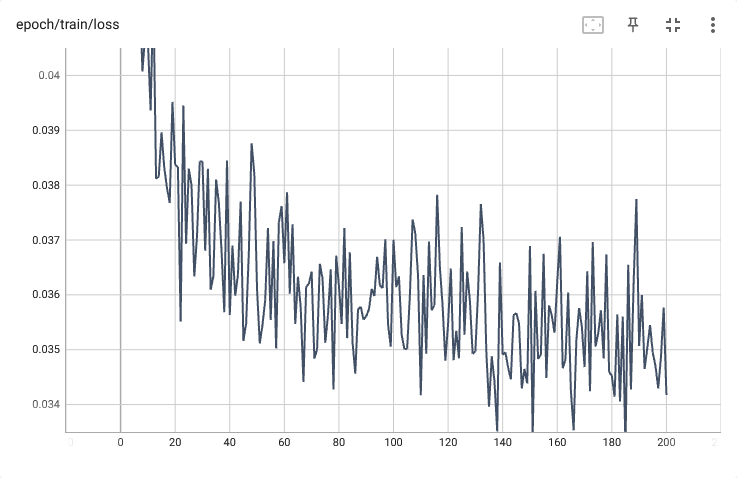
\includegraphics[width=\textwidth]{chapters/figures/3_md/loss/pr-1em-v850-train-loss.png}
      \caption{pr 1em v850 Train loss}
      \label{fig:md:1em-v850-train-loss}
  \end{subfigure}
  \hfill
  \begin{subfigure}[b]{0.4\textwidth}
      \centering
      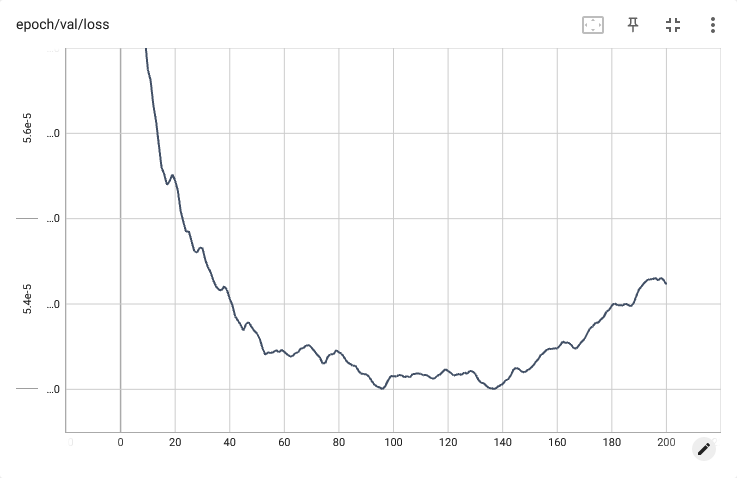
\includegraphics[width=\textwidth]{chapters/figures/3_md/loss/pr-1em-v850-val-loss.png}
      \caption{pr 1em v850 Val loss}
      \label{fig:md:1em-v850-val-loss}
  \end{subfigure}
  \hfill
  \caption{Train and validation loss for various iterations of the diffusion model.}
  \label{fig:md:loss}
\end{figure}


\section{Inputs}

\subsection{Perfect vs imperfect}

\subsection{Avoid 925hPa}

Some datasets used in the literature use 925hPa-level variables as coarse inputs \parencite[e.g.][]{}.
However, for our domain this includes grid cells for which this pressure level is often below the surface (e.g. upland areas) leading to odd values in the data at this level.

\subsection{Feature selection}

We demonstrate the value of various input variables for the diffusion model by comparing the performance of the model with different sets of input variables.

\subsubsection{lr pr}

\subsubsection{V850}

Chan et al

\subsubsection{V4th}

\subsubsection{V4thT4th}

T for CCS

\subsubsection{V4thT4thS4th}

\subsubsection{pslV4thT4th}

\subsubsection{pslV4thT4thS4th}

\section{Transfer to GCM inputs}